\subsection{Installazione applicazione esterna a Grafana}
In questa sezione verrà descritta la modalità con cui è possibile installare l'applicazione esterna.

\subsubsection{Installazione degli strumenti}
\paragraph{Strumenti}\mbox{}\\ [1mm]
Gli strumenti necessari per installare correttamente l'applicativo esterno sono:
\begin{itemize}
    \item \textbf{Node.js}: runtime Javascript che permette di eseguire codice Javascript fuori da un browser, l'installazione di npm (Node Package Manager) non è richiesta in quanto viene installato automaticamente durante l'installazione di Node.js;
    \item \textbf{Git}: sistema di versionamento distribuito.
\end{itemize}
\mbox{}\\ [1mm]
Questi strumenti possono essere installati con diverse metodologie; tuttavia presenteremo un esempio per non appesantire questo manuale con informazioni non strettamente pertinenti all'applicativo esterno.

\paragraph{Node}\mbox{}\\ [1mm]
Per installare il runtime Javascript Node.js si può visitare il sito \url{https://nodejs.org}. Qui è possibile trovare il download di Node.js per tutti i sistemi operativi. Alternativamente, nei sistemi operativi basati su Linux, è possibile utilizzare lo strumento di gestione dei pacchetti fornito per installare quelli del runtime Node.js. Di seguito un esempio per sistemi operativi basati Debian/Ubuntu: \\
\begin{verbatim}
    apt-get install nodejs
\end{verbatim}

\paragraph{Git}\mbox{}\\ [1mm]
Per installare il sistema di versionamento distribuito Git si può visitare la pagina web \href{https://git-scm.com/downloads}. Qui è possibile trovare il download per MacOS, Windows e sistemi operativi basati su Linux/Unix. Alternativamente, nei sistemi operativi basati su Linux, è possibile utilizzare lo strumento di gestione dei pacchetti fornito.  Di seguito un esempio per sistemi operativi basati Debian/Ubuntu: \\
\begin{verbatim}
    apt-get install git
\end{verbatim}

\subsubsection{Installazione dell'applicazione}
L'installazione dell'applicazione è suddivisa in due passaggi che descriviamo in dettaglio nei prossimi paragrafi.
\begin{enumerate}
    \item clonare la repository da GitHub;
    \item installare le dipendenze.
\end{enumerate}

\paragraph{Clonare la repository da GitHub}\mbox{}\\ [1mm]
Per clonare la repository dell'applicazione, aprire un terminale e usare il comando \texttt{cd} per muovervi in una cartella a vostra scelta. Quindi eseguite il comando \verb|git clone https://github.com/VRAM-Software/grafana_prediction.git| per clonare la repository principale del nostro prodotto.
Infine per spostarsi nella cartella che contiene il codice sorgente dell'applicativo esterno si usa il comando: \verb|cd ./prediction_configuration_utility|.
\\
\\
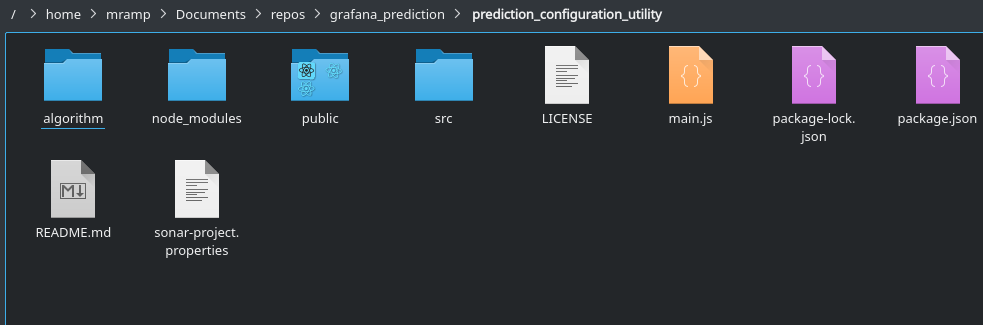
\includegraphics[width=\textwidth,height=\textheight,keepaspectratio]{img/directoryProject.png}


\paragraph{Installare le dipendenze}\mbox{}\\ [1mm]
Per il corretto funzionamento dell'applicazione è necessario installare tutte le dipendenze elencate nel file \texttt{package.json}. Per farlo eseguire il comando \texttt{npm install} da terminale nella cartella \verb|prediction_configuration_utility|. I pacchetti che verranno installati si suddividono in dipendenze e dipendenze sviluppatore, di seguito verrano spiegate le due categorie.
\\
\\
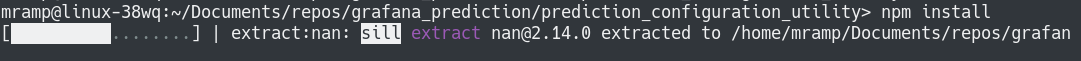
\includegraphics[width=\textwidth,height=\textheight,keepaspectratio]{img/packageInstallation.png}

\subparagraph*{Dipendenze}\mbox{}\\ [1mm]
Nella seguente tabella sono elencate tutte le dipendenze necessarie per la corretta esecuzione dell'applicazione.
\rowcolors{2}{gray!25}{gray!15}
	\setcounter{table}{0}
	\begin{longtable} {
		>{}p{65mm} 
		>{}p{30mm}
		}
    \rowcolor{gray!50}
    \textbf{Pacchetto} & \textbf{Versione} \TBstrut \\ [2mm]
    \verb|@testing-library/jest-dom| & \verb|^4.2.4|  \TBstrut \\ [2mm]
    \verb|@testing-library/react| & \verb|^9.3.2| \TBstrut \\ [2mm]
    \verb|@testing-library/user-event| & \verb|^7.1.2| \TBstrut \\ [2mm]
    \verb|csvtojson| & \verb|2.0.10| \TBstrut \\ [2mm]
    \verb|d3| & \verb|^5.15.0| \TBstrut \\ [2mm]
    \verb|electron-is-dev| & \verb|^1.1.0| \TBstrut \\ [2mm]
    \verb|ml-modules|\footnote{Il pacchetto \texttt{ml-modules} usato nel nostro progetto è una versione modificata dell'ononimo pacchetto} & \verb|0.1.0| \TBstrut \\ [2mm]
    \verb|react| & \verb|^16.13.0| \TBstrut \\ [2mm]
    \verb|react-dom| & \verb|^16.13.0| \TBstrut \\ [2mm]
    \verb|react-router-dom| & \verb|^5.1.2| \TBstrut \\ [2mm]
    \verb|react-scripts| & \verb|3.4.0| \TBstrut \\ [2mm]
    \end{longtable}
    
\subparagraph*{Dipendenze sviluppatore}\mbox{}\\ [1mm]
Nella seguente tabella sono elencate tutte le dipendenze necessarie per la corretta esecuzione dell'applicazione durante lo sviluppo della stessa.
\rowcolors{2}{gray!25}{gray!15}
	\setcounter{table}{0}
	\begin{longtable} {
		>{}p{65mm} 
		>{}p{30mm}
		}
    \rowcolor{gray!50}
    \textbf{Pacchetto} & \textbf{Versione} \TBstrut \\ [2mm]
    \verb|electron| & \verb|^8.02| \TBstrut \\ [2mm]
    \verb|electron-packager| & \verb|^14.2.1| \TBstrut \\ [2mm]
    \verb|coveralls| & \verb|^3.0.9| \TBstrut \\ [2mm]
    \end{longtable}
    \mbox{}\\ [1mm]
Seguendo i due passaggi descritti nei precedenti paragrafi, l'applicazione esterna è installata correttamente.
